\documentclass{beamer}

%% \documentclass[handout]{beamer}
%% % use this with the [handout] option to create handouts for the audience
%% \usepackage{pgfpages}
%% \pgfpagesuselayout{2 on 1}[a4paper,border shrink=5mm]

\mode<presentation>
{
  \usetheme{Diku}
% set this to your preferences:
%  \setbeamercovered{invisible}
  \setbeamercovered{transparent}
}

\usepackage{graphicx}
\usepackage{epic}

\usepackage{amsmath}
\usepackage{amssymb}
\usepackage{amsthm}

\newcommand{\basetop}[1]{\vtop{\vskip-1ex\hbox{#1}}}
\newcommand{\source}[1]{\let\thefootnote\relax\footnotetext{\scriptsize\textcolor{kugray1}{Source: #1}}}

% for coloured code citation in text:
\usepackage{fancyvrb}

%%%%%%%%%%%%%%%%%%%%%%%%%%%%%%%%%
%%%%%    code sections   %%%%%%%%
%%%%%%%%%%%%%%%%%%%%%%%%%%%%%%%%%

% code highlighting commands in own block
\DefineVerbatimEnvironment{code}{Verbatim}{fontsize=\scriptsize}
\DefineVerbatimEnvironment{icode}{Verbatim}{fontsize=\scriptsize}

% Fancy code with color commands:
\DefineVerbatimEnvironment{colorcode}%
        {Verbatim}{fontsize=\scriptsize,commandchars=\\\{\}}

%%%%%%%%%%%%%%%%%%%%%%%%%%%%%%%%%%
%%%%%    some coloring    %%%%%%%%

%% use "DIKU green" from our color theme for \emph
%\renewcommand{\emph}[1]{\textcolor{structure}{#1}}
%% use some not-too-bright red for an \emp command
%\definecolor{DikuRed}{RGB}{130,50,32}
%\newcommand{\emp}[1]{\textcolor{DikuRed}{ #1}}
%\definecolor{CosGreen}{RGB}{10,100,70}
%\newcommand{\emphh}[1]{\textcolor{CosGreen}{ #1}}


\definecolor{Red}{RGB}{220,50,10}
\definecolor{Blue}{RGB}{0,51,102}
\definecolor{Yellow}{RGB}{102,51,0}
\definecolor{Orange}{RGB}{178,36,36}
\definecolor{Grey}{RGB}{180,180,180}
\definecolor{Green}{RGB}{20,120,20}
\definecolor{Purple}{RGB}{160,50,100}
\newcommand{\red}[1]{\textcolor{Red}{{#1}}}
\newcommand{\blue}[1]{\textcolor{Blue}{{#1}}}
\newcommand{\yellow}[1]{\textcolor{Yellow}{{#1}}}
\newcommand{\orange}[1]{\textcolor{Orange}{{#1}}}
\newcommand{\grey}[1]{\textcolor{Grey}{{#1}}}
\newcommand{\green}[1]{\textcolor{Green}{{#1}}}
\newcommand{\purple}[1]{\textcolor{Purple}{{#1}}}




% use "DIKU green" from our color theme for \emph
\renewcommand{\emph}[1]{\textcolor{structure}{#1}}
% use some not-too-bright red for an \emp command
\definecolor{DikuRed}{RGB}{130,50,32}
\newcommand{\emp}[1]{\textcolor{DikuRed}{ #1}}
\definecolor{CosGreen}{RGB}{10,100,70}
\newcommand{\emphh}[1]{\textcolor{CosGreen}{ #1}}
\definecolor{CosBlue}{RGB}{55,111,122}
\newcommand{\emphb}[1]{\textcolor{CosBlue}{ #1}}
\definecolor{CosRed}{RGB}{253,1,1}
\newcommand{\empr}[1]{\textcolor{CosRed}{ #1}}

\newcommand{\mymath}[1]{$ #1 $}
\newcommand{\myindx}[1]{_{#1}}
\newcommand{\myindu}[1]{^{#1}}

\newtheorem{mydef}{Definition}
\newtheorem{mytheo}{Theorem}
\newtheorem{mylemma}{Lemma}

%%%%%%%%%%%%%%%%%%%%

\title[Map-Reduce]{Pure-Functional, Map-Reduce\\Programming Abstraction}

\author[C.~Oancea]{Cosmin E. Oancea {\tt cosmin.oancea@diku.dk}}

\institute{Department of Computer Science (DIKU)\\University of Copenhagen}


\date[Sept 2014]{September 2014 PMPH Lecture Notes}


\begin{document}

% \titleslide command WRAPS THIS SEQUENCE
%% % Set background to front page
%% \usebackgroundtemplate{
\includegraphics[width=\paperwidth,height=\paperheight]{front}}
%% {
%% \begin{frame}[plain]
%%   \titlepage
%% \end{frame}
%% }
\titleslide


\begin{frame}[fragile]
	\tableofcontents
\end{frame}

%%%%%%%%%%%%%%%%%%%%%%%%%%%%%%%%%%%%%%%
%%%%%%%% CONTENT STARTS HERE %%%%%%%%%%
%%%%%%%%%%%%%%%%%%%%%%%%%%%%%%%%%%%%%%%

\section{List Homomorphism}

\subsection{First Theorem of Homomorphisms}

\begin{frame}[fragile,t]
\frametitle{Math Preliminaries: Monoid \& Homomorphism}

\begin{mydef}[Monoid]\label{MonoidDef}\vspace{-1ex}
Assume set $S$ and $\odot : S \times S \rightarrow S$.
\emp{$(S, \odot)$ is called a Monoid} if it satisfies the following two axioms:\\
\emp{(1) Associativity:} $\forall x,y,z\in S$ we have 
    $(x \odot y) \odot z \equiv x \odot (y \odot z)$ and\\
\emp{(2) Identity Element:} $\exists e \in S$ such that $\forall a \in S$, %we have
    $e \odot a \equiv a \odot e \equiv a$.\\\medskip

($(S,\odot)$ is called a group if it also satisfies that any element is 
    invertible, i.e., 
    $\forall a, \exists a^{-1}$ such that 
    $a\odot a^{-1}\equiv a^{-1}\odot a\equiv e$.)
\end{mydef}

E.g., $(\mathbb{N},+)$, $(\mathbb{Z},\times)$, $(\mathbb{L}_T,++)$, where\\
        $\mathbb{L}_T$ denotes lists of elements of type $T$,
        and $++$ list concatenation. 

\begin{mydef}[Monoid Homomorphism]\label{HomDef}\vspace{-1ex}
\emp{A monoid homomorphism} from monoid $(S,\oplus)$ to monoid $(T,\odot)$
is a function $h : S \rightarrow T$ such that $\forall u, v\in S$,
\emp{$h(u\oplus v) \equiv h(u)\odot h(v)$}.
\end{mydef}

%\alert{This has a shape similar to divide and conquer algorithms!}

\end{frame}



\begin{frame}
  \frametitle{List Homomorphism (LH)}

\begin{itemize}
    \item Work with finite lists, where {\tt ++} denotes concatenation:
        \begin{itemize}
            \item {\tt [1,2,3,4] ++ [5,6,7,8] = [1,2,3,4,5,6,7,8]},
            \item neutral element $e_{\tt++}$ is the empty list, 
                i.e., {\tt [1,2]++[] = [1,2]},
            \item later we will look at them as \emph{vectors} rather 
                    than \alert{linked lists}.
        \end{itemize}
%    \item Motivation: a large class of list-homomorphic function have 
%            {\em efficient data-parallel} (map-reduce style) implementations!
\end{itemize}

\begin{mydef}[List Homomorphism]\label{LHomDef}
$h :: [T_1] \rightarrow T_2$ over finite lists is a {\em list homomorphism}
if there exists a(n associative) binary operator $\odot :: T_2 \rightarrow T_2 \rightarrow T_2$,
such that: \\
$\mbox{ }\mbox{ }\mbox{ }\mbox{ }\mbox{ }\mbox{ }\mbox{ }\mbox{ }\mbox{ }$
\emp{$h \mbox{ } (x{\tt ++}y) = (h\mbox{ }x)\mbox{ }\odot\mbox{ }(h\mbox{ }y)$} \\
We denote $h = hom \mbox{ }(\odot) \mbox{ }f\mbox{ }e$, where $f(x) = h([x])$ 
and $e = h([])$. 
\end{mydef}

\begin{itemize}
    \item If the program is well behaved, i.e., same result
            for any {\tt x++y} splitting of the input list, 
            then $(T_2,\odot)$ is necessarily a Monoid.\smallskip

    \item Shape is similar to a divide and conquer algorithm, where 
            {\tt h(x)} and {\tt h(y)} can be computed in parallel 
            and results can be merged. 
\end{itemize}
\end{frame}


\begin{frame}[fragile,t]
  \frametitle{List Homomorphism (LH) Examples}

%Those functions that promote through list concatenation ({\tt ++}):
%$h\mbox{ }(x {\tt ++} y) = (h\mbox{ }x) \odot (h\mbox{ }y)$. More precise:

\begin{mydef}[List Homomorphism]\label{LHomDef}
$h :: [T_1] \rightarrow T_2$ over finite lists is a {\em list homomorphism}
if there exists an associative binary operator $\odot :: T_2 \rightarrow T_2 \rightarrow T_2$,
such that: \\
$\mbox{ }\mbox{ }\mbox{ }\mbox{ }\mbox{ }\mbox{ }\mbox{ }\mbox{ }\mbox{ }$
\emp{$h \mbox{ } (x{\tt ++}y) = (h\mbox{ }x)\mbox{ }\odot\mbox{ }(h\mbox{ }y)$} \\
We denote $h = hom \mbox{ }(\odot) \mbox{ }f\mbox{ }e$, where $f\mbox{ }x = h\mbox{ }[x]$ and $e = h\mbox{ }[]$. 
\end{mydef}

\begin{block}{Examples of List Homomorphisms, id x = x is the identity function}
\vspace{-2ex}
\begin{columns}
\column{0.45\textwidth}
\begin{colorcode}[fontsize=\scriptsize]
-- \emp{len} = \emp{hom (+) one 0}, one x = 1
len :: [T] -> Integer
len []     = \emp{0}
len [x]    = \emp{1}
\emph{len} (x++y) = (\emph{len} x) \emp{+} (\emph{len} y)

-- \emph{flatten} = \emp{hom (++) id []}
flatten :: [[T]] -> [T]
flatten []     = \emp{[]}
flatten [x]    = \emp{x}
\emph{flatten} (x++y) = (\emph{flatten} x) \emp{++} 
                 (\emph{flatten} y)
\end{colorcode}
\column{0.45\textwidth}
\begin{colorcode}[fontsize=\scriptsize]
-- \emph{maxList} = \emp{hom (max) id \mymath{-\infty}} 
maxList :: [Int] -> Int
maxList []     = \emp{\mymath{-\infty}}
maxList [x]    = \emp{x}
\emph{maxList} (x++y) = (\emph{maxList} x) \emp{`max`} 
                 (\emph{maxList} y)
-- Assume p :: T -> Bool given,
-- \emph{all\mymath{\myindx{p}}} = \emp{hom (&&) p True}
all\mymath{\myindx{p}} :: [T] -> Bool
all\mymath{\myindx{p}} []     = \emp{True}
all\mymath{\myindx{p}} [x]    = \emp{p x} 
\emph{all\mymath{\myindx{p}}} (x++y) = (\emph{all\mymath{\myindx{p}}} x) \emp{&&} (\emph{all\mymath{\myindx{p}}} y)
\end{colorcode}
\end{columns}
\end{block}

%Definition~\ref{LHomDef} implies

\end{frame}


\begin{frame}[fragile,t]
  \frametitle{Exercise: Implement the above LHs in Haskell}

\begin{block}{Implementation Sample for all$_p$:} 
\begin{colorcode}[fontsize=\scriptsize]
import System.Environment -- access to arguments etc.
-- helper to simulate (x++y) pattern
split :: [a] -> ([a], [a])
split []  = ([],[] )
split [x] = ([],[x]) 
split xs  = let mid = (length xs) `div` 2  in  (take mid xs, drop mid xs)

-- \emph{all\mymath{\myindx{p}}} \mymath{\equiv} \emph{alln p} = \emp{hom (\mymath{\wedge}) p True}
\emph{alln} :: (a -> Bool) -> [a] -> Bool
\emph{alln p} []     = True
\emph{alln p} [x]    = p x
\emph{alln p} xs     = let (x, y) = split xs   in   (\emph{alln p} x) && (\emph{alln p} y)

----- Compile with: ghc -O2 -o test LHegHaskell.hs -----
main :: IO()
main = do args <- getArgs
          let inp = if null args then [0,2,4,6] else read (head args)
              p x = x `mod` 2 == 0
              res = alln p inp  
          putStrLn ("Computed: " ++ show res)
\end{colorcode}
\end{block}
\end{frame}



\begin{frame}[fragile,t]
  \frametitle{Map, Reduce, and Scan Types and Semantics}

\begin{itemize}
    \item \emp{\tt map~::~($\alpha\rightarrow\beta$)~$\rightarrow$~[$\alpha$]$~\rightarrow$~[$\beta$]}\\
    \emph{\tt map f [x$_1,\ldots, $x$_n$] = [f(x$_1$),$\ldots$, f(x$_n$)]},\\  
        i.e., \emp{\tt{}x$_i$~::~$\alpha, \forall i$}, and 
        \emp{\tt f~::~$\alpha\rightarrow\beta$}.\medskip

    \item \emp{{\tt reduce~::~($\alpha$~$\rightarrow$~$\alpha$~$\rightarrow$~$\alpha$)~$\rightarrow$~$\alpha$~$\rightarrow$~[$\alpha$]~$\rightarrow$~$\alpha$}}\\
        \emph{\tt reduce $\odot$~e~[x$_1$,x$_2$,..,x$_n$]~=~e$\odot$x$_1\odot$x$_2\odot\ldots\odot$x$_n$},\\
        i.e., \emp{{\tt{}e::$\alpha$, x$_i$~::~$\alpha, \forall i$}}, and 
        \emp{\tt $\odot$~::~$\alpha\rightarrow\alpha\rightarrow\alpha$}.\medskip

    \item \emp{{\tt scan$^{exc}$~::~($\alpha$~$\rightarrow$~$\alpha$~$\rightarrow$~$\alpha$)~$\rightarrow$~$\alpha$~$\rightarrow$~[$\alpha$]~$\rightarrow$~[$\alpha$]}}\\
        \emph{\tt scan$^{exc}~\odot$~e~[x$_1$,$\ldots$,x$_n$]~=~[e,e$\odot$x$_1$,$\ldots$,e$\odot$x$_1\odot\ldots$x$_{n-1}$]}\\
        i.e., \emp{{\tt{}e::$\alpha$, x$_i$~::~$\alpha, \forall i$}}, and 
        \emp{\tt $\odot$~::~$\alpha\rightarrow\alpha\rightarrow\alpha$}.\medskip

    \item \emp{{\tt scan$^{inc}$~::~($\alpha$~$\rightarrow$~$\alpha$~$\rightarrow$~$\alpha$)~$\rightarrow$~$\alpha$~$\rightarrow$~[$\alpha$]~$\rightarrow$~[$\alpha$]}}\\
        \emph{\tt scan$^{inc}~\odot$~e~[x$_1$,$\ldots$,x$_n$]~=~[e$\odot$x$_1$,$\ldots$,e$\odot$x$_1\odot\ldots$x$_{n}$]}\\
        i.e., \emp{{\tt{}e::$\alpha$, x$_i$~::~$\alpha, \forall i$}}, and 
        \emp{\tt $\odot$~::~$\alpha\rightarrow\alpha\rightarrow\alpha$}.

\end{itemize}

\end{frame}


\begin{frame}[fragile,t]
  \frametitle{1st List-Homomorphism Theorem [Meertens]}

\begin{mytheo}[1st List Homomorphism Theorem (Meertens)]\label{LHomTh1}
Any homomorphism \emp{$h = hom \ (\odot) \ f \ e$} can be written 
as the composition of a reduce and a map: \\
\emp{$\ \ \ \ \ \ \ \ \ h = hom \ (\odot) \ f \ e_{\odot} \ = \ (reduce \ (\odot) \ e_{\odot}) \ . \ (map \ f)$} \\
Conversely, each such composition is a homomorphism. \\
\end{mytheo}

\bigskip

Theorem tells how to parallelize LHs based on {\tt map-reduce} skeletons.
%Note that $\mbox{ }map\mbox{ }f \equiv map_f\mbox{ }\mbox{ }$ and 
%$\mbox{ }\mbox{ }hom\mbox{ }(\odot)\mbox{ }id\mbox{ }e_{\odot} \equiv red_{\odot}$

\bigskip

\begin{block}{Map-Reduce Definition for the Discussed LH Examples} \vspace{-1.5 ex}
\begin{columns}
\column{0.5\textwidth}
\begin{colorcode}[fontsize=\scriptsize]
-- len = hom \emp{(+)} \emph{one} \emp{0}, one x = 1
len = \emp{(reduce (\emp{+}) 0)} . \emph{(map one)}

-- sum = hom \emp{(+)} \emph{id} \emp{0}, id x = x
sum = \emp{(reduce (+) 0)} . \emph{(map id)}

-- flatten = hom \emp{(++)} \emph{id} \emp{[]},
flatten = \emp{(reduce (++) [])} . \emph{(map id)}
\end{colorcode}
\column{0.45\textwidth}
\begin{colorcode}[fontsize=\scriptsize]
-- maxList = hom \emp{(max)} \emph{id} \emp{\mymath{-\infty}}
maxList = \emp{(reduce (max) (\mymath{-\infty})}) . 
          \emph{(map id)}

-- all\mymath{\myindx{p}} = hom \emp{(&&)} \emph{p} \emp{True}
all\mymath{\myindx{p}} = \emp{(reduce (&&) True)} . 
       \emph{(map p)}

\end{colorcode}
\end{columns}
\end{block}

\end{frame}



\begin{frame}[fragile,t]
  \frametitle{List Homomorphism Invariants}

\begin{mytheo}[List-Homomorphism Promotions]\label{LHomInv}
Given unary functions $f$, $g$ and an associative binary operator $\odot$ then:\\
%$\mbox{ }$ \\
\emp{1.}$\ \ ({\tt map} \ f) \ . \ ({\tt map} \ g) \ \ \equiv \ \ {\tt map} \ (f \ . \ g)$\\
$\mbox{ }$ \\
\emp{2.}$\ \ ({\tt map} \ f) \ . \ ({\tt reduce} \ ({\tt ++}) \ []) \ \equiv \ ({\tt reduce} \ ({\tt ++}) \ []) \ . \ ({\tt map} \ ({\tt map} \ f) )$ \\
$\mbox{ }$ \\
\emp{3.}$\ \ ({\tt reduce} \ \odot \ e_{\odot}) \ . \ ({\tt reduce} \ (++) \ []) \ \equiv$\\
$ \ \ \ \ \ \ \ \ \ \ \ \ \ \ \ \ \ \ \ \ \ \ \ \ \ \ \ \ \ \ \ \ \ \ \
({\tt reduce} \ \odot \ e_{\odot}) \ . \ ({\tt map} \ ({\tt reduce} \ \odot \ e_{\odot}) )$
\end{mytheo}

%  

\begin{itemize}
    \item \emp{2. 3. $\Rightarrow$ code generation:} list is segmented, 
            segments are distributed on different processors, 
            computation proceeds locally on each processor, 
            and the local results are reduced. 
    \item \emph{2. 3. $\Leftarrow$ flattening optimization}: 
            uncovers more parallelism
    \item e.g., map f [1..4] = (map f) . (red ++) [[1,2],[3,4]] =$^{prom1}$ \alert{?}           
%(red ++) . (map (map f)) [[1,2], [3,4]] = \\red ++ [map f [1,2], map f [3,4]]
\end{itemize}

\end{frame}


\begin{frame}[fragile,t]
  \frametitle{Optimizing Map-Reduce Computation}

\begin{mytheo}[Optimized Map Reduce]\label{MapRed}
Assume {\tt distr$_p :: [\alpha] \rightarrow [[\alpha]]$}
distributes a list into $p$ sublists, each containing about 
the same number of elements. Denoting  
${\tt redomap }\ \odot \ f \ e_{\odot} \ \equiv \ ({\tt reduce} \ \odot \ e_{\odot}) \ . \ (map \ f)$, the equality holds:\\\bigskip

\emp{${\tt redomap} \ \odot \ f \ e_{\odot} \ \ \equiv$}\\
\emp{$\ \ \ \ \ \ \ \ \ \ \ \ \ \ \ \ \ \ \ ({\tt reduce} \ \odot \ e_{\odot}) \ . \ ({\tt map} \ ({\tt redomap} \ \odot \ f \ e_{\odot})) \ . \ {\tt distr}_p$}
\end{mytheo}

\begin{itemize}
    \item \alert{Prove it!}
    \item \emph{Hint: $({\tt reduce} \ (++) \ []) \ . \ {\tt distr}_p \ \ \equiv \ \ id$, hence}
    \item \emph{${\tt redomap }\ \odot \ f \ e_{\odot} \ \equiv$\\ $\ \ \ \ ({\tt reduce} \ \odot \ e_{\odot}) \ . \ (map \ f) \ . \ ({\tt reduce} \ (++) \ []) \ . \ {\tt distr}_p$}
\end  {itemize}

\end{frame}
%    \item  Motivation: a large class of list-homomorphic 
%           function have {\em efficient data-parallel} 
%           (map-reduce style) implementations!


%%%%%%%%%%%%%%%%%%%%%%%%%%%%%%%%%%%%%%%%%%%%%
%%%%%%%%%%%%%%%%%%%%%%%%%%%%%%%%%%%%%%%%%%%%%
%%%%%%%%%%%%%%%%%%%%%%%%%%%%%%%%%%%%%%%%%%%%%
\subsection{Near Homomorphisms (Cole)}

\begin{frame}[fragile]
	\tableofcontents[currentsubsection]
\end{frame}


\begin{frame}[fragile,t]
  \frametitle{Near Homomorphisms [Cole]}

\emp{M. Cole, ``Parallel Programming, List Homomorphisms and the Maximum Seqment Sum Problem''.} 
\bigskip

\emph{Intuitive Idea}: a non-homomorphic problem $g$ can be sometimes ``lifted'' to a 
homomorphism one $f$, by computing a ``baggage'' of extra information. 

\bigskip

The initial problem can be obtained via a projection from the (homomorphic) 
result: $g\mbox{ }=\pi\mbox{ }.\mbox{ }f$

\bigskip

\emp{Maximum-Segment Sum ({\tt mss}) Problem}: \\
given a list of integers, find the contiguous segment of the list 
whose members have the largest sum among all such segments. Return the sum (only).

\bigskip

E.g., {\tt mss} [1, -2, 3, 4, -1, 5, -6, 1] = 11 \\
(the corresponding segment is [3, 4, -1, 5]). 

\end{frame}


\begin{frame}[fragile,t]
  \frametitle{Maximum Segment Sum}

\begin{block}{Incorrect list-homomorphism implementation}
\begin{colorcode}
mss []       = 0
mss (x{\tt ++}\mbox{ }y) = (mss x) \mymath{\uparrow} (mss y) -- x \mymath{\uparrow} y = if (x > y) then x else y
\end{colorcode}
\end{block} 

\smallskip

\alert{Incorrect:} {\tt (mss [1,-2,3,4])\mymath{\uparrow}(mss [-1,5,-6,1]) $\equiv$ 7 \mymath{\uparrow} 4 $\equiv$ 7} \\
\emph{The correct result} of {\tt (mss [1, -2, 3, 4, -1, 5, -6, 1])} \emph{is} 11, corresponding to segment [3, 4, -1, 5].

\bigskip

\emph{The segment of interest may lie partly in {\tt x} and partly in {\tt y}.} 
To construct a homomorphism we need to compute extra information:\pause
\begin{itemize}
    \item maximum concluding segment: {\tt mcs x = mcs [1,-2,3,4] = 7}
    \item maximum initial segment: {\tt mis y = mis [-1,5,-6,1] = 4}
    \item total segment sum: {\tt ts [1,-2,3,4] = 6}
    \item {\tt mis (x++y) = (mis x) $\uparrow$ ((ts x)+(mis y))}, similar for {\tt mcs}    
    \item {\tt mss (x++y) = (mss x) $\uparrow$ (mss y) $\uparrow$ ((mcs x) + (mis y))}
\end{itemize}
\end{frame}


\begin{frame}[fragile,t]
  \frametitle{Maximum-Segment Sum = Near Homomorphism}

\begin{block}{Correct Solution -- Test it in Haskell!}
\begin{colorcode}
-- \mymath{x\mbox{ }\uparrow\mbox{ }y = if(x >= y) then x else y}
(mssx, misx, mcsx, tsx) \mymath{\odot} (mssy, misy, mcsy, tsy) = (
        (mssx\mymath{\mbox{ }\uparrow\mbox{ }}mssy\mymath{\mbox{ }\uparrow\mbox{ }}(mcsx+misy),
         misx\mymath{\mbox{ }\uparrow\mbox{ }}(tsx+misy),
        (mcsx+tsy)\mymath{\mbox{ }\uparrow\mbox{ }}mcsy,
         tsx + tsy
    )

f x = (x\mymath{\mbox{ }\uparrow\mbox{ }}0, x\mymath{\mbox{ }\uparrow\mbox{ }}0, x\mymath{\mbox{ }\uparrow\mbox{ }}0, x)

\emph{emss = (reduce \mymath{\odot} (0,0,0,0)) . (map f)}

\emp{mss  = \mymath{\pi\myindx{1}} . emss}
       where \mymath{\pi\myindx{1}} (a, _, _, _) = a 
\end{colorcode}
\end{block} 

\smallskip

The baggage: three extra integers per communication stage and \\ 
a constant number of integer operations.

Optimal time and work complexity with $N/log(N)$ processors.

\end{frame}


\begin{frame}[fragile,t]
  \frametitle{Longest Satisfying Segment Problems}

\begin{itemize}
    \item Class of problems which requires to find the longest segment of a list
            for which some property holds
    \item e.g., longest sequence of zeroes, of the same number, sorted  
    \item How about longest sequence whose sum is 0?
    \item For the latter any correct solution needs to access the complete list, giving 
            sequential implementation without any parallelism, \\ e.g., {\tt lsum0 [4,1,1] $\odot$ lsum0[-2,5,1]}.
\end{itemize}

\bigskip

\begin{block}{Restrict the Shape of the Predicate:}
\begin{colorcode}
p []           = True
p [x]          = ...
p [x, y]       = ...
p [x : y : zs] = (p [x,y]) \mymath{\wedge} p (y : zs)
\end{colorcode}
\end{block} 

\end{frame}


\begin{frame}[fragile,t]
  \frametitle{Longest Satisfying Segment Problems}

\begin{block}{Restrict the Shape of the Predicate:}
\begin{colorcode}
zeroes [x]   = x == 0           same [x]   = True     sorted [x]   = True
zeroes [x,y] =  (zeroes [x])    same [x,y] = x == y   sorted [x,y] = x <= y
              \mymath{\wedge} (zeroes [y])
\end{colorcode}
\end{block} 

\bigskip
Extra Baggage:
\begin{itemize}
    \item As before, the \emp{length} of the longest initial/concluding  satisfying segments ({\tt lis}/{\tt lcs}),
            and the total list length ({\tt tl}).
    \item When considering the concatenation of the {\tt (lcs, lis)} pair, it is not guaranteed that the
            result satisfies the predicate \\
            e.g., {\tt (sorted x) $\wedge$ (sorted y) $\not\Rightarrow$ sorted x++y}.  
    \item Hence store the {\em last} element of {\tt lcs} and the {\em first} element of {\tt lis},
    \item and compute whether {\tt (lcs x)} is {\em connected} to {\tt (lis y)}, \\ i.e., {\tt p [lastx,firsty] == True}
    \item Boolean indicating whether the whole list satisfies {\tt p} ({\tt ok}).
\end{itemize}
\end{frame}

\begin{frame}[fragile,t]
  \frametitle{Longest Satisfying Segment Problem: Exercise}

\begin{block}{Exercise: fill in the blanks, test in Haskell for zeroes/same/sorted}
\begin{colorcode}
(lssx, lisx, lcsx, tlx, firstx, lastx, okx) \mymath{\odot}
(lssy, lisy, lcsy, tly, firsty, lasty, oky) 

  = (newlss, newlis, newlcs, tlx+tly, firstx, lasty, newok)
     where
        connect = ...
        newlss  = ...
        newlis  = ... 
        newlcs  = ... 
        newok   = ...

f x = (xmatch, xmatch, xmatch, 1, x, x, p [x])
    where xmatch = if (p [x]) then 1 else 0

\emph{elss = (reduce (\mymath{\odot}) (0,0,0,0,0,0,True)) . (map f)}

\emp{lss  = \mymath{\pi\myindx{1}} . elss}
       where \mymath{\pi\myindx{1}} (a, _, _, _, _, _, _) = a         
\end{colorcode}
\end{block} 

%lssx \mymath{\uparrow} lssy \mymath{\uparrow} (if connect then ... else 0)
%+ (if okx \mymath{\wedge} connect then ... else 0)
%+ (if oky \mymath{\wedge} connect then ... else 0)
%okx \mymath{\wedge} oky \mymath{\wedge} connect

\end{frame}



%\begin{frame}[fragile,t]
%  \frametitle{Longest Satisfying Segment Problem -- Solution}
%
%\begin{block}{Longest Satisfying Segment Solution}
%\begin{colorcode}
%(lssx, lisx, lcsx, tlx, firstx, lastx, okx) \mymath{\odot}
%(lssy, lisy, lcsy, tly, firsty, lasty, oky) 
%
%  = (newlss, newlis, newlcs, tlx+tly, firstx, lasty, newok)
%     where
%        connect = p [lastx, firsty]
%        newlss  = lssx \mymath{\uparrow} lssy \mymath{\uparrow} (if connect then lcsx+lisy else 0)
%        newlis  = lisx + (if okx \mymath{\wedge} connect then lisy else 0)
%        newlcs  = lcsy + (if oky \mymath{\wedge} connect then lcsx else 0)
%        newok   = okx \mymath{\wedge} oky \mymath{\wedge} connect
%
%f x = (xmatch, xmatch, xmatch, 1, x, x, p [x])
%    where xmatch = if (p [x]) then 1 else 0
%
%-- In Haskell write \emp{red \mymath{(\odot)\mbox{ }e\myindx{\odot}}}, where \mymath{e\myindx{\odot} = (0,0,0,0,0,0,True)}
%\emph{elss = (red \mymath{\odot}) . (map f)}
%
%\emp{lss  = \mymath{\pi\myindx{1}} . elss}
%       where \mymath{\pi\myindx{1}} (a, _, _, _, _, _, _) = a         
%\end{colorcode}
%\end{block} 
%
%\end{frame}

%%%%%%%%%%%%%%%%%%%%%%%%%%%%%%%%%%%%%%%
%%%%%%%%%%%%%%%%%%%%%%%%%%%%%%%%%%%%%%%
%%%%%%%%%%%%%%%%%%%%%%%%%%%%%%%%%%%%%%%
\subsection{Scan as a Distributable Homomorphism}
\begin{frame}[fragile]
	\tableofcontents[currentsubsection]
\end{frame}

\begin{frame}[fragile,t]
  \frametitle{All Homomorphism Are Efficient?}

If the combine operator involves concatenation then does
map-reduce provides efficient parallelization? 

\begin{block}{Merge Sort} \vspace{-1.5 ex}
\begin{columns}
\column{0.45\textwidth}
\begin{colorcode}[fontsize=\scriptsize]
-- merge two sorted lists
merge :: Ord T => [T] -> [T] -> [T]
merge [] y  = y
merge x  [] = x
merge (x:xs) (y:ys) = 
  if ( x <= y ) 
  then x : merge xs (y:ys)
  else y : merge (x:xs) ys 
\end{colorcode}
\column{0.45\textwidth}
\begin{colorcode}[fontsize=\scriptsize]
-- \emph{mSort} = \emp{hom merge [.] []}
-- [.] x = [x]  
\emph{mSort} :: Ord T => [T] -> [T]
\emph{mSort} []     = \emp{[]}
\emph{mSort} [x]    = \emp{[x]}
\emph{mSort} (x++y) = (\emph{mSort} x) \emp{`merge`}  
               (\emph{mSort} y)
\end{colorcode}
\end{columns}
\end{block}

In the naive merged sort, the {\tt merge} reduction operator
traverses sequentially the whole list, hence this map-reduce 
does not give efficient parallelization!

\end{frame}


\begin{frame}[fragile,t]
  \frametitle{Distributable Homomorphism (DH)}

\begin{itemize}
    \item DH: a class of homomorphisms that allows efficient parallel
            implem even if concatenation appears in the reduction operator.
    \item Requires that the length of the list is a power of 2,
            and at every step the list is split in half.
    \item {\tt zipWith :: [$\alpha$] $\rightarrow$ [$\beta$] $\rightarrow$ [$\gamma$]},\\
          {\tt zipWith $\odot$ [x$_1$,$\ldots$,x$_n$] [y$_1$,$\ldots$,y$_n$] $\equiv$ [x$_1\odot$y$_1$,$\ldots$,x$_n\odot$y$_n$]}
\end{itemize}
\vspace{-1ex}
\begin{mydef}[Distributable Homomorphism (DH)]\label{DistribHom}
Given two associative binary operators $\oplus$ and $\otimes$ we define operator \\
$\mbox{ }\mbox{ }\mbox{ }\mbox{ }$ 
{\tt dhop} ::  % (a$\rightarrow$a$\rightarrow$a) $\rightarrow$ (a$\rightarrow$a$\rightarrow$a) $\rightarrow$ 
                        [a] $\rightarrow$ [a] $\rightarrow$ [a] \\
$\mbox{ }\mbox{ }\mbox{ }\mbox{ }$ 
{\tt dhop}  u v = (zipWith $\oplus$ u v) ++ (zipWith $\otimes$ u v) \\  % $\oplus$ $\otimes$
\vspace{1ex}
We write $\oplus\updownarrow\otimes$ for the LH with combine operator {\tt dhop} $\oplus$ $\otimes$\\
$\mbox{ }\mbox{ }\mbox{ }\mbox{ }$ 
$\oplus\updownarrow\otimes$ [a]   $\mbox{ }\mbox{ }\mbox{ }\mbox{ }\mbox{ }\mbox{ }$    = [a] \\
$\mbox{ }\mbox{ }\mbox{ }\mbox{ }$ 
$\oplus\updownarrow\otimes$ (x ++ y) = ($\oplus\updownarrow\otimes$ x) {\tt `dhop`} ($\oplus\updownarrow\otimes$ y) \\
\vspace{1ex}
Function $h :: [T] -> [T]$ is a distributable homomorphism iff $h = \oplus\updownarrow\otimes$ for some binary associative
operators  $\oplus$ and $\otimes$.
\end{mydef}

\end{frame}


\begin{frame}[fragile,t]
  \frametitle{Distributed Reduce is a DH}

\begin{columns}
\column{0.4\textwidth}
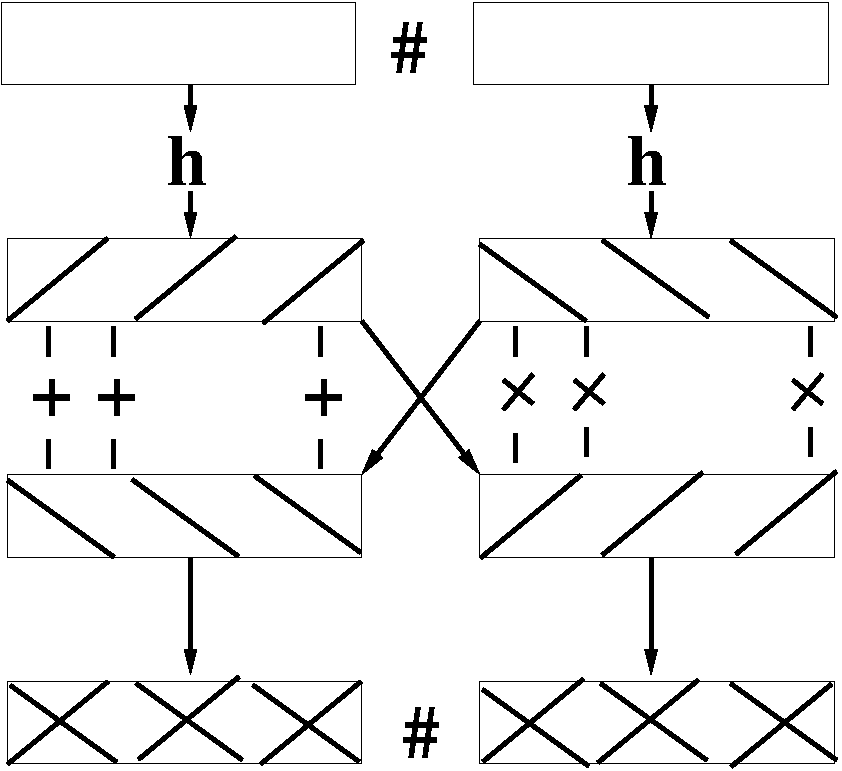
\includegraphics[height=25ex]{Figures/DH}
\column{0.6\textwidth}\vspace{-3ex}
\begin{itemize}
    \item {\tt dhop u v = (zipWith $\oplus$ u v) ++}\\ 
          {\tt~~~~~~~~~~~(zipWith $\otimes$ u v)}
    \item {\tt $\oplus\updownarrow\otimes$ (x ++ y) = ($\oplus\updownarrow\otimes$ x)}\\
          {\tt~~~~~~~~~~`dhop` ($\oplus\updownarrow\otimes$ y)} 
\end{itemize}
\end{columns}

\begin{itemize}
    \item For example, distributed reduction: 
        {\tt distrRed ($\odot$) e$_\odot$ x = }\\
        {\tt [reduce $\odot$ e$_{\odot}$ x,$\ldots$, reduce $\odot$ e$_{\odot}$ x]}
    \item is a DH: distrRed $\odot$ = $\odot\updownarrow\odot$
\end{itemize}

\end{frame}


\begin{frame}[fragile,t]
  \frametitle{Scan is a DH}

\begin{columns}
\column{0.4\textwidth}
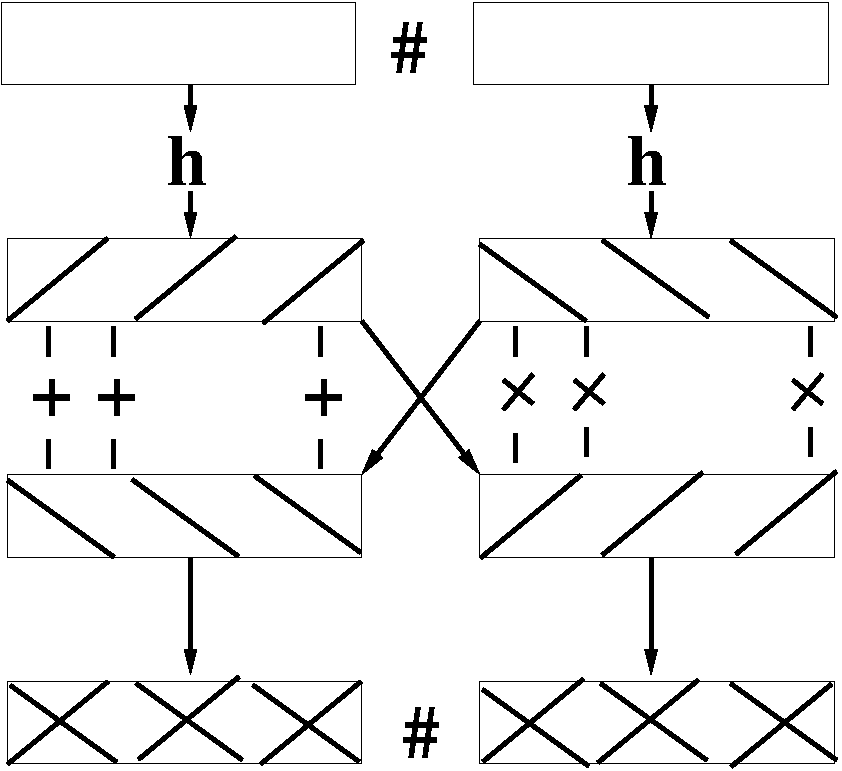
\includegraphics[height=25ex]{Figures/DH}
\column{0.6\textwidth}\vspace{-3ex}
\begin{itemize}
    \item {\tt dhop u v = (zipWith $\oplus$ u v) ++}\\ 
          {\tt~~~~~~~~~~~(zipWith $\otimes$ u v)}
    \item {\tt $\oplus\updownarrow\otimes$ (x ++ y) = ($\oplus\updownarrow\otimes$ x)}\\
          {\tt~~~~~~~~~~`dhop` ($\oplus\updownarrow\otimes$ y)} 
\end{itemize}
\end{columns}


\begin{itemize}
    \item ${\tt scan} \ \odot \ {\tt e}_{\odot} \ {\tt(x++y)} = S_1~\oslash~S_2~=~S_1$
            {\tt ++ (map ($\odot$ s) $S_2$)},\\ 
            where $S_1${\tt = scan $\odot$ e$_{\odot}$ x},
                  $S_2${\tt = scan $\odot$ e$_{\odot}$ y}, and {\tt s=last $S_1$}\medskip
 
    \item {\tt dhScan $\odot$ e$_{\odot}$ = (map $\pi_1$) . ($\oplus\updownarrow\otimes$) . (map pair)},\\
            where {\tt $\pi_1$ (a,b) = a,~~~~pair a = (a,a)},\\
            {\tt (s$_1$,r$_1$) $\oplus$ (s$_2$,r$_2$) = (s$_1$, r$_1$ $\odot$ r$_2$)}\\
            {\tt (s$_1$,r$_1$) $\otimes$ (s$_2$,r$_2$) = (r$_1$ $\odot$ s$_2$, r$_1$ $\odot$ r$_2$)}
\end{itemize}

\end{frame}


%%%%%%%%%%%%%%%%%%%%%%%%%%%%%%%%%%%%%%%
%%%%%%%%%%%%%%%%%%%%%%%%%%%%%%%%%%%%%%%
%%%%%%%%%%%%%%%%%%%%%%%%%%%%%%%%%%%%%%%
\section{Nested Data Parallelism}

\begin{frame}[fragile]
	\tableofcontents[currentsection]
\end{frame}

\subsection{Implementation of Reduce and Scan Bulk Operations}

\begin{frame}[fragile,t]
  \frametitle{Parallel Random Access Machine (PRAM)}

PRAM focuses exclusively on parallelism and ignores issues
related to synchronization and communication:
\begin{itemize}
    \item[1] $p$ processors connected to shared memory
    \item[2] each processor has an unique id (index) $i$, $1 \leq i \leq p$
    \item[3] SIMD execution, each parallel instruction requires unit time,
    \item[4] each processor has a flag that controls whether it is active
                in the execution of an instruction.
\end  {itemize}


\begin{columns}
\column{0.6\textwidth}
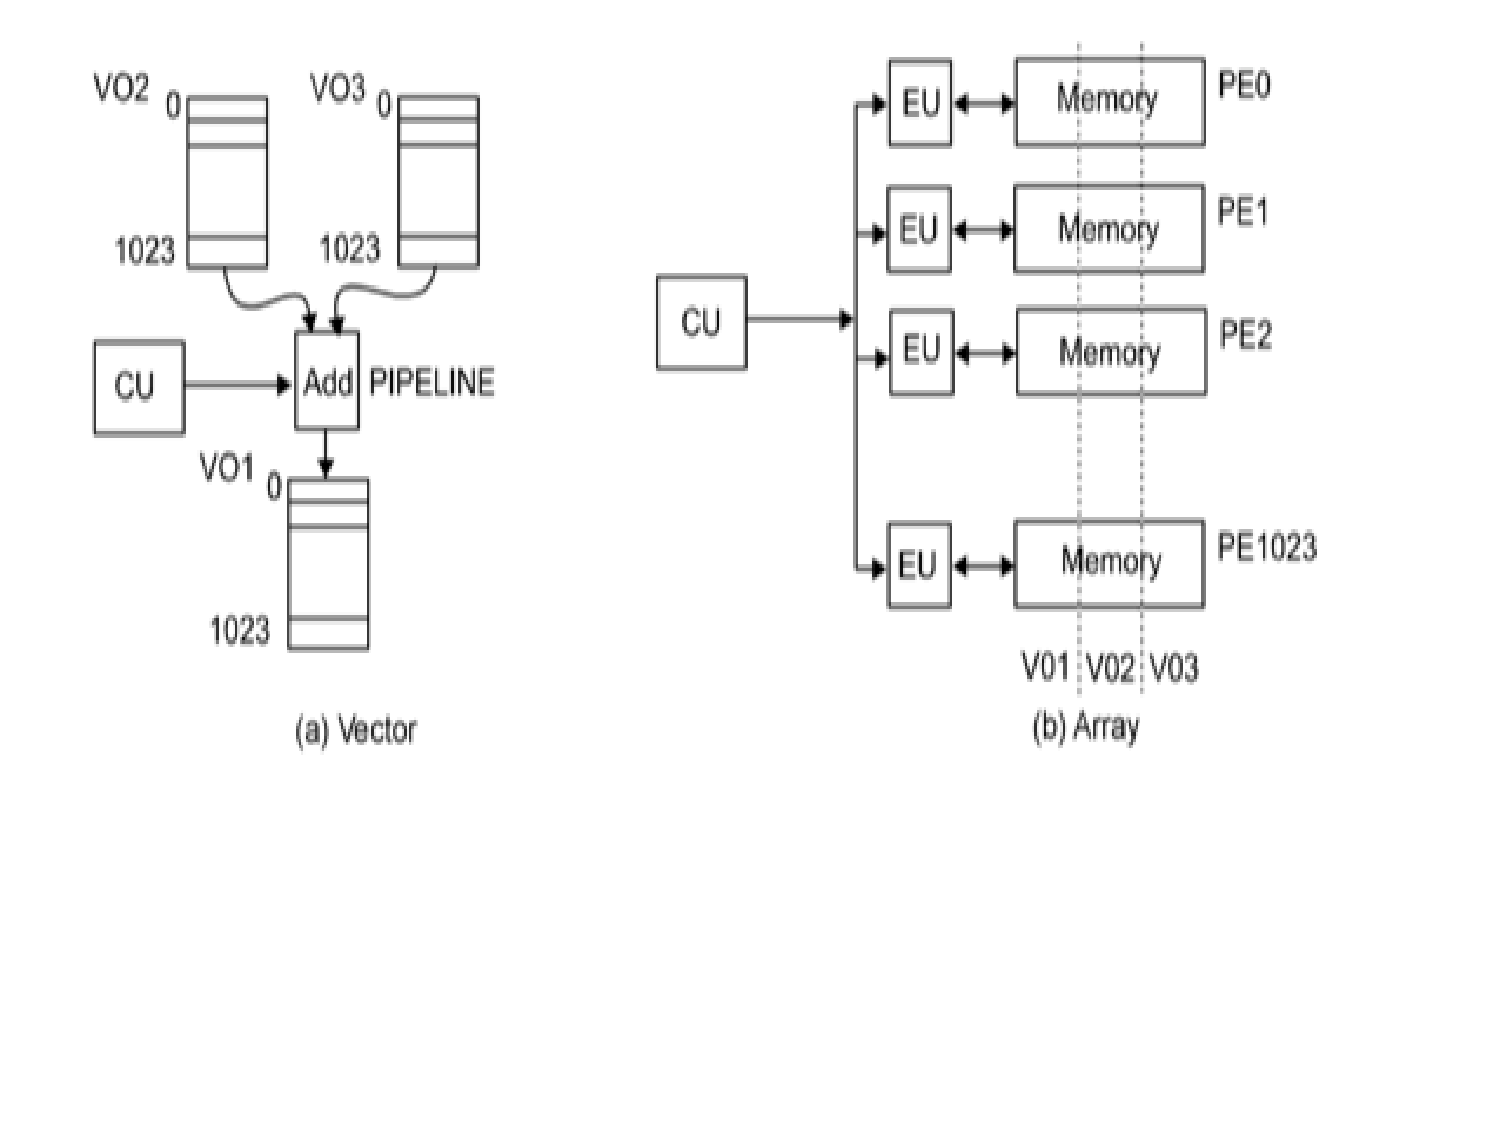
\includegraphics[height=37ex]{Ch1Figs/VectorMachine}
\column{0.5\textwidth}\vspace{-15ex}
\begin{itemize}
    \item \emp{Work Time Algorithm (WT):}
    \item \emp{Work Complexity W(n)}: is the total \# of ops performed,
    \item \emp{Depth/Step Complexity D(n)}: is the \# of sequential steps.\medskip
    \item \emph{WT $\longrightarrow$ PRAM algorithm\\by Brent Theorem}.
\end{itemize}
\end{columns}

\end{frame}


\begin{frame}
  \frametitle{Reducing in Parallel}

\begin{columns}
\column{0.6\textwidth}
        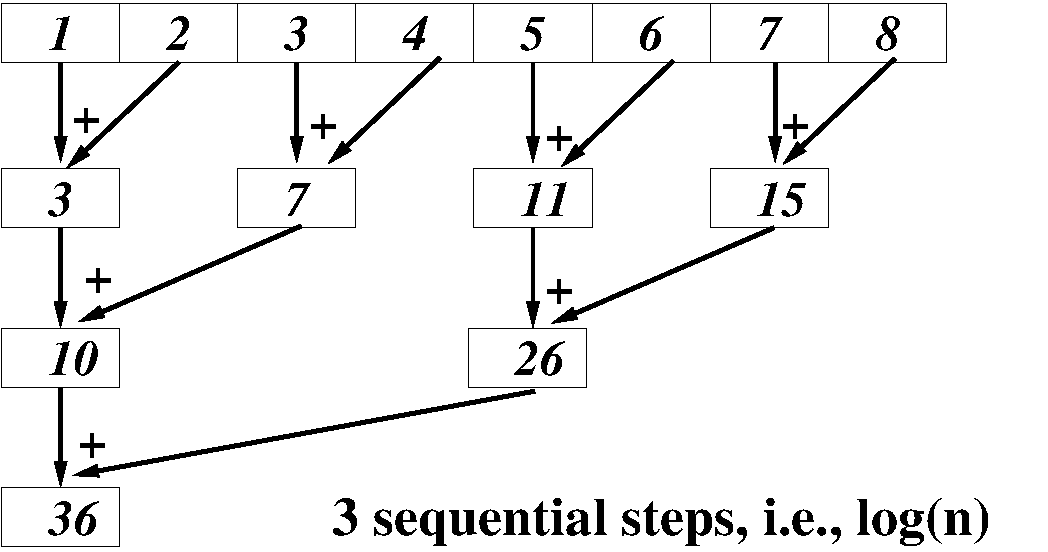
\includegraphics[height=22ex]{Figures/ReduceEg.pdf} 
\column{0.5\textwidth}
Reducing an array of length {\tt n} with {\tt  n/2} processors requires:
\begin{itemize}
    \item work $W(n) = n$ and 
    \item depth $D(n) = lg \ n$, i.e., number of sequential steps.
    \item optimized runtime with $P$ processors: \emph{$(n/P) + lg \ P$.}
\end  {itemize}
\end{columns}

\begin{mytheo}[Brent Theorem]\label{BrentTh}
A Work-Time Algorithm of depth $D(n)$ and work $W(n)$ can be
simulated on a $P$-processor PRAM in time complexity T such that:\\\bigskip
\emp{$\ \ \ \ \ \ \ \ \ \ \ \ \ \ \ \ \frac{W(n)}{P} \leq T < \frac{W(n)}{P} + D(n)$}
\end{mytheo}

\end{frame}


\begin{frame}[fragile,t]
  \frametitle{Reduce: Algorithm and Complexity}


\begin{columns}
\column{0.5\textwidth}
\begin{colorcode}[fontsize=\scriptsize]
Input:  array A of n=2\mymath{\myindu{k}} elems of type T
        \mymath{\oplus::T\times T\rightarrow T} associative
Output: S = \mymath{\oplus\myindx{j=1}\myindu{n} a\myindx{j}}

1.  \emph{forall i \mymath{\in} 1 : n do}
2.    B[i] \mymath{\leftarrow} A[i]
3.  \emph{enddo}

4.  \emp{for h = 1 to k do}
5.    \emph{forall i \mymath{\in} 1 : n by 2\mymath{\myindu{h}} do} 
6.      B[i] \mymath{\leftarrow} B[i] \mymath{\oplus} B[i+2\mymath{\myindu{h-1}}]
7.    \emph{enddo}
8.  \emp{enddo}
9.  S \mymath{\leftarrow} B[1]  
\end{colorcode}
\column{0.59\textwidth}
\begin{itemize}
    \item $D_{1-3}(n) = \Theta(1)$, $W_{1-3}(n) = \Theta(n)$,
    \item $D_{5-7}(n) = \Theta(1)$, $W_{5-7}(n,h) = \Theta(n/2^h)$,
    \item $D_{4-8}(n) = k \times D_{5-7}(n) = \Theta(lg \ n)$
    \item $W_{4-8}(n) = \sum_{h=1}^k W_{5-7}(n,h) = $\\
          $\Theta(\sum_{h=1}^k (n/2^h) ) = \Theta(n)$
    \item $D_{9}(n) = \Theta(1)$, $W_{9}(n) = \Theta(1)$,\bigskip
    \item \emp{$D(n) = \Theta(lg \ n), W(n) = \Theta(n)$!}
\end{itemize}
\end{columns}
\bigskip

%\mymath{\frac{n}{2\myindu{h}}} do}

\begin{center}  
\emp{$\frac{n-1}{P} \leq  Runtime < \frac{n-1}{P} + lg \ n$}
\end{center}


\end{frame}


\begin{frame}[fragile,t]
  \frametitle{Parallel Scan with Associative Operator $\oplus$}
\bigskip

\begin{columns}
\column{0.4\textwidth}
        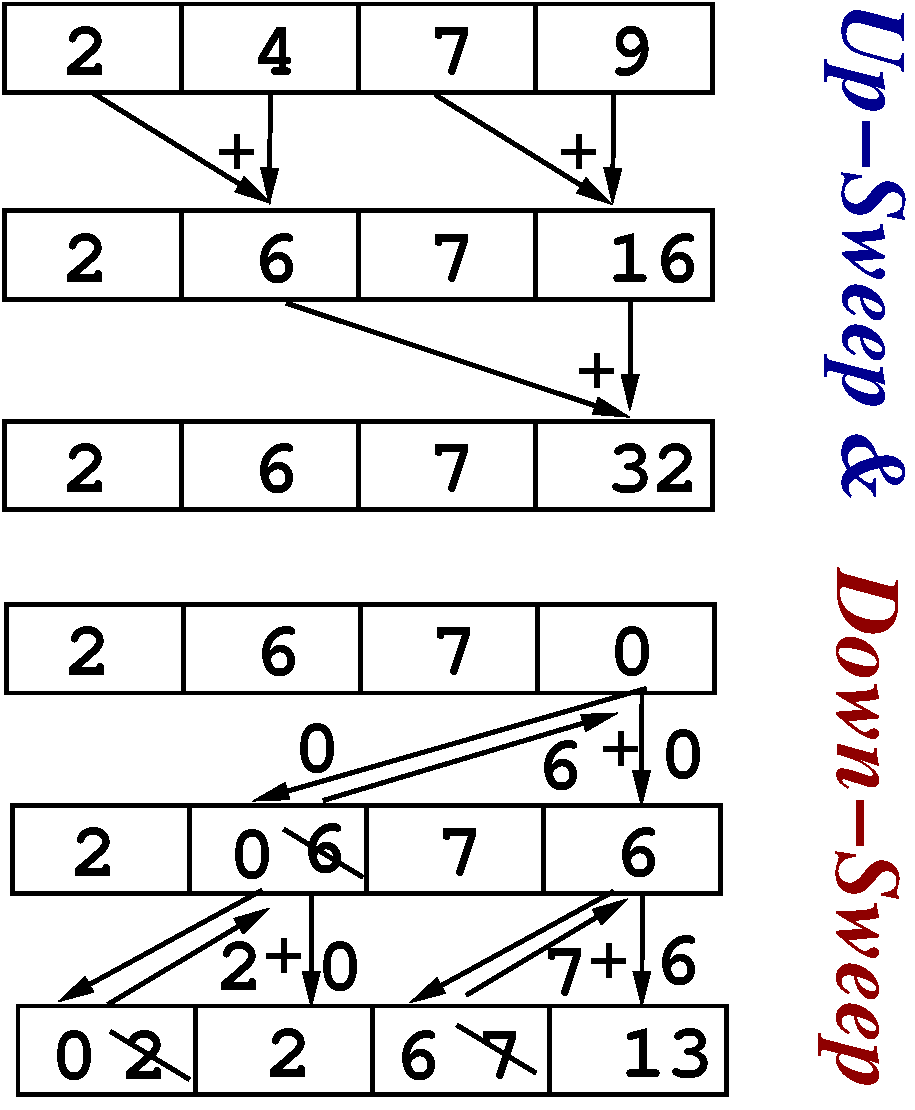
\includegraphics[height=33ex]{Figures/ScanEg.pdf} 
\column{0.6\textwidth}
Two Steps:
\begin{itemize}
    \item \blue{Up-Sweep:} similar with reduction
    \item Root is replaced with neutral element.
    \item \emp{Down-Sweep:} 
    \begin{itemize}
        \item the left child sends its value to parent and 
                updates its value to that of parent.
        \item the right-child value is given by $\oplus$ 
                applied to the left-child value and
                the (old) value of parent.
        \item note that the right child is in fact the parent,
                i.e., in-place algorithm.
    \end  {itemize}
\end  {itemize}
\end{columns}


\end{frame}



\begin{frame}[fragile,t]
  \frametitle{Parallel Scan Algorithm And Complexity}
\bigskip

\begin{columns}
\column{0.5\textwidth}
\begin{colorcode}[fontsize=\scriptsize]
Input:  array A of n=2\mymath{\myindu{k}} elems of type T
        \mymath{\oplus::T\times T\rightarrow T} associative
Output: B = \mymath{[0, a\myindx{1}, a\myindx{1}\oplus{}a\myindx{2},\ldots,\oplus\myindx{j=1}\myindu{n-1} a\myindx{j}]}

1.  \emph{forall i \mymath{\in} 1 : n do}
2.    B[i] \mymath{\leftarrow} A[i]
3.  \emph{enddo}

4.  \emp{for h = 1 to k do} // up-sweep
5.    \emph{forall i \mymath{\in} n : 1 by -2\mymath{\myindu{h}} do} 
6.      B[i] \mymath{\leftarrow} B[i] \mymath{\oplus} B[i-2\mymath{\myindu{h-1}}]
7.    \emph{enddo}
8.  \emp{enddo}
9.  B[n] = 0

10. \emp{for h = k downto 1 do} // down-sweep
11.   \emph{forall i \mymath{\in} n : 1 by -2\mymath{\myindu{h}} do} 
12.     tmp = B[i]
13.     B[i] \mymath{\leftarrow} B[i] \mymath{\oplus} B[i-2\mymath{\myindu{h-1}}]
14.     B[i-2\mymath{\myindu{h-1}}] = tmp
15.   \emph{enddo}
16. \emp{enddo}
\end{colorcode}
\column{0.59\textwidth}
\begin{itemize} 
    \item The code show exponentials for clarity, but those can
            be computed by one multiplication/division operation
            each sequential iteration.
    \item \emp{$D(n) = \Theta(lg \ n), W(n) = \Theta(n)$!}
    \item Similar reasoning as with reduce.
\end{itemize}
\end{columns}


\end{frame}

%%%%%%%%%%%%%%%%%%%%%%%%%%%%%%%%%%%%%%%%%
%%%%%%%%%%%%%%%%%%%%%%%%%%%%%%%%%%%%%%%%%
\subsection{Other Second-Order Bulk Operators}

\begin{frame}[fragile,t]
  \frametitle{Zip, ZipWith}

\begin{itemize}
    \item \emph{\tt zip :: [$T_1$] $\rightarrow$ [$T_2$] $\rightarrow$ [($T_1$,$T_2$)]}
    \item \emp{\tt zip [a$_1$,$\ldots$,a$_n$] [b$_1$,$\ldots$,b$_m$] $\equiv$ [(a$_1$,b$_1$),\ldots,(a$_q$,b$_q$)]},
            where {\tt q = min(m,n)}.
    \item \emph{\tt unzip :: [($T_1$,$T_2$)] $\rightarrow$ ([$T_1$],[$T_2$])}
    \item \emp{\tt unzip [(a$_1$,b$_1$),\ldots,(a$_n$,b$_n$)]$\equiv$([a$_1$,$\ldots$,a$_n$],[b$_1$,$\ldots$,b$_n$])},\medskip

    \item In some sense {\tt zip} is syntactic sugar, for example one could work with the
            tuple of array representation, e.g.,
    \item \emp{\tt mapT :: (($\alpha_1$,$\ldots$,$\alpha_m$)$\rightarrow$($\beta_1$,$\ldots$,$\beta_n$)) $\rightarrow$}\\ 
          \emp{\tt~~~~~~~~~[$\alpha_1$] $\rightarrow\ldots\rightarrow$ [$\alpha_m$] $\rightarrow$ ([$\beta_1$],$\ldots$,[$\beta_n$]])}
    \item \emph{\tt mapT f $\equiv$ unzip$^n$ . map f . zip$^n$}\medskip

    \item {\tt zipWith :: [$\alpha_1$] $\rightarrow$ [$\alpha_2$] $\rightarrow$ [$\beta$]}
    \item {\tt zipWith $\odot$ [a$_1$,$\ldots$,a$_n$] [b$_1$,$\ldots$,b$_n$] $\equiv$ [a$_1\odot$b$_1$,$\ldots$,a$_n\odot$b$_n$]}
    \item {\tt zipWith $\odot$ $\equiv$ map ($\backslash$(u,v) $\rightarrow$ u $\odot$ v) . zip}
\end  {itemize}

\end{frame}

\begin{frame}[fragile,t]
  \frametitle{Permute, Split, Filter}

\begin{itemize}
    \item Operator to permute an array based on a list (array) of indices:
    \item \emph{permute :: [$\alpha$] $\rightarrow$ [Int] $\rightarrow$ [$\alpha$]}, e.g.,\\
           A (data vector) {\tt~= [a0,~a1,~a2,~a3,~a4,~a5]}\\
           I (index vector){\tt~~= [3,~~2,~~0,~~4,~~1,~~5~]}\\
           permute A I     {\tt~~~~= [a2,~a4,~a1,~a0,~a3,~a5]}\medskip

    \item Operator to {\tt split} a list (array) at a certain index:
    \item \emph{\tt split :: Int $\rightarrow$ [$\alpha$] $\rightarrow$ ([$\alpha$],[$\alpha$])}
    \item \emp{\tt split i [a$_0$,$\ldots$,a$_{i-1}$,$\ldots$ a$_n$] $\equiv$ ([a$_0$,$\ldots$,a$_{i-1}$],[a$_i$,$\ldots$,a$_{n}$])}\medskip
 
    \item \emph{\tt filter :: ($\alpha\rightarrow$Bool) $\rightarrow$ [$\alpha$] $\rightarrow$ [$\alpha$]}
    \item \emp{\tt filter cond X $\equiv$ [b$_0$,$\ldots$,b$_{m}$]}, such that 
                {\tt b$_j, \forall j\in\{0\ldots m\}$,} are all the elements of array 
                {\tt X} that evaluate to {\tt True} under condition {\tt cond}, i.e., {\tt (cond b$_j$) $\equiv$ True}.\medskip

    \item \alert{Can {\tt filter} be implemented via {\tt map} and {\tt reduce} (and {\tt scan})?}

\end  {itemize}

\end{frame}

\begin{frame}[fragile,t]
  \frametitle{Filter: Implementation based on Map and Scan}

%\mymath{\backslash}

\begin{columns}
\column{0.59\textwidth}
\begin{colorcode}[fontsize=\scriptsize]
//filter cond X, where 
// cond :: \mymath{\alpha\rightarrow}Bool
let cs = map cond X
    flags = map (\mymath{\backslash}f->if f then 1 
                          else 0) cs
    isT   = scan\mymath{\myindu{inc}} (+) 0 flags
    i     = last isT

    nflags= map (\mymath{\backslash}f->if f then 0 
                          else 1) cs
    isF   = (map (+ i) . scan\mymath{\myindu{inc}} (+) 0) 
            nflags

    inds  = map (\mymath{\backslash} (c,iT,iF) -> 
                    if c then iT-1 else iF-1) 
                (zip3 cs isT isF)
in  permute X inds
\end{colorcode}
\column{0.4\textwidth}
\begin{colorcode}[fontsize=\scriptsize]
Assume X = [5,4,2,3,7,8], and 
cond is T(rue) for even nums.
cs    = [F, T, T, F, F, T]
flags = [0, 1, 1, 0, 0, 1]

isT   = [0, 1, 2, 2, 2, 3]
i     = 3

nflags= [1, 0, 0, 1, 1, 0]

isF   = [4, 4, 4, 5, 6, 6]


inds  = [3, 0, 1, 4, 5, 2]


Result is: [4,2,8,5,3,7] 
\end{colorcode}
\end{columns}

\end{frame}

%%%%%%%%%%%%%%%%%%%%%%%%%%%%%%%%%%%%%%%%%%%%%
%%%%%%%%%%%%%%%%%%%%%%%%%%%%%%%%%%%%%%%%%%%%%
%%%%%%%%%%%%%%%%%%%%%%%%%%%%%%%%%%%%%%%%%%%%%

%\begin{frame}[fragile,t]
%  \frametitle{Bird-Meertens Formalism (BMF)}
%
%BMF: small collection of (i) second-order functions on lists,
%    (ii) algebraic identities and theorems, 
%    and (iii) a concise notation. 
%
%\begin{block}{BMF Notation:}
%\begin{columns} 
%\column{0.1\textwidth}
%$\mbox{ }$ \\
%${\tt id}$ \\ 
%${\tt .}$\\
%$ \oplus, \otimes, \odot$ \\
%$ {\tt zip} \mbox{ } \odot$\\
%$\mbox{ }$\\
%$ {\tt map} \mbox{ } f$\\
%$\mbox{ }$\\
%$ {\tt red} \mbox{ } \odot$\\ %\mbox{ }e_{\odot}$
%$\mbox{ }$\\
%$\mbox{ }$\\
%$ {\tt scan}\mbox{ }\odot$\\ %\mbox{ }e_{\odot}
%$\mbox{ }$ \\
%$\mbox{ }$
%\column{0.8\textwidth}
%identity function, i.e., ${\tt id} : T \rightarrow T, {\tt id}\mbox{ }x = x$ \\
%backward functional composition: $(f\mbox{ }.\mbox{ }g)\mbox{ }x = f\mbox{ }(g\mbox{ }x)$ \\
%binary associative operators, $\odot :: T \rightarrow T \rightarrow T$ \\
%application of $\odot$ to a pair of equal-length lists: \\
%${\tt zip}\mbox{ }\odot\mbox{ }[x_1,..,x_n]\mbox{ }[y_1,..,y_n]\mbox{ }=\mbox{ }[x_1\odot y_1,..,x_n\odot y_n]$. \\
%$f :: T_{1} \rightarrow T_{2}$, ${\tt map} :: [T_{1}] \rightarrow [T_{2}]$, \\
%${\tt map} \mbox{ }f\mbox{ } [x_{1},..,x_{n}] \mbox{ }=\mbox{ }[f\mbox{ }x_{1},..,f\mbox{ }x_{n}]$ \\
%reduce with binary associative operator $\odot$, ${\tt red}::(T \rightarrow T \rightarrow T) \rightarrow [T] \rightarrow T$, $e_{\odot} = red\mbox{ }\odot\mbox{ }[]$ \\
%${\tt red} \odot [a] = a$, ${\tt red} \odot (x {\tt ++} y) = (red \odot x) \odot (red \odot y)$ \\
%prefix sum: ${\tt scan}::(T \rightarrow T \rightarrow T) \rightarrow [T] \rightarrow [T] $, \\ %${\tt scan} \odot [x_1,..,x_n] = [x_1, x_1\odot x_2,..,x_1\odot x_2\odot .. \odot x_n]$ 
%\end{columns}
%\end{block}
%
%%${\tt sum} = {\tt red}\mbox{ }(+)$ \\
%%${\tt flatten} = {\tt red}\mbox{ }({\tt ++})$ \\
%
%%$ {\tt id} $\\
%%the identity function
%%$<f_1, .., f_n>$
%%zipped tupling: \mymath{f\myindx{i} :: [a] -> [a], i=1,..,n}  
%\end{frame}









%%%%%%%%%%%%%%%%%%%%%%%%%%%%%%%%%%%%%%%
%%%%%%%% LECTURE NUMBER 2 %%%%%%%%%%%%%
%%%%%%%%%%%%%%%%%%%%%%%%%%%%%%%%%%%%%%%





%%%%%%%%%%%%%%%%%%%%%%%%%%%%%%%%%%%%%%%
%%%%%%%% CONTENT ENDS   HERE %%%%%%%%%%
%%%%%%%%%%%%%%%%%%%%%%%%%%%%%%%%%%%%%%%

\end{document}
